\documentclass[a4paper,twoside, 10pt]{article}
\usepackage[%CJKbookmarks=true,
	unicode=true,
	hyperindex=true,
	pdfstartview=FitH,
	bookmarksnumbered=true,	%注释掉此行则书签前没有数字编号
	bookmarksopen=true,  	%注释掉此行则默认不展开书签
	colorlinks=true, 	%注释掉此项则交叉引用为彩色边框(将colorlinks和pdfborder同时注释掉)
	pdfborder=001,   	%注释掉此项则交叉引用为彩色边框
	citecolor=red
]{hyperref}

\usepackage{graphicx}		%图像宏包
\usepackage{amsmath}		%ams数学宏包
\usepackage{algorithm}		% algorithm package
\usepackage{algpseudocode}	% algorithmicx package is included therein
\usepackage{simplewick}

\usepackage[utf8]{inputenc}
\usepackage[english]{babel}
\usepackage{amsthm}
\DeclareMathOperator{\Tr}{Tr}

\newtheorem{theorem}{Theorem}
\theoremstyle{wick}
\newtheorem*{wick}{Wick's Theorem}

\newtheorem{lemma}[theorem]{Lemma}

\usepackage{extarrows}		%长等号、等号上下
\usepackage{textcomp}		%摄氏度
\usepackage{multirow,makecell}
\usepackage{mhchem}
\usepackage{pifont}
\usepackage{subfig}		%subfloat

\newcommand{\mr}{\mathrm}
\newcommand{\tr}{\textrm}
\newcommand{\tN}{\tr{N}}
\newcommand{\md}{\mathrm{d}}
\newcommand{\mi}{\mathrm{i}}
\newcommand{\me}{\mathrm{e}}
\newcommand{\mg}{\mathrm{g}}
\newcommand{\br}{\bm{r}}
\newcommand{\bR}{\bm{R}}
\newcommand{\bt}{\bm{\tau}}
\newcommand{\bk}{\bm{k}}
\newcommand{\bK}{\bm{K}}
\newcommand{\ba}{\bm{a}}
\newcommand{\bb}{\bm{b}}
\newcommand{\bG}{\bm{G}}
\newcommand{\bq}{\bm{q}}
\newcommand{\bB}{\bm{B}}
\newcommand{\bx}{\bm{x}}
\newcommand{\vD}{\varDelta}
\newcommand{\Ao}{\mathring{\mr{A}}}
\newcommand{\tc}{\textcelsius}
\newcommand{\oo}{$\ddot{\mathrm{o}}$}
\newcommand{\hh}{\hat{E}}
\newcommand{\mcH}{\mathcal{H}}
\newcommand{\mcS}{\mathcal{S}}
\newcommand{\mcM}{\mathcal{M}}
\newcommand{\psik}{\psi_{\bm{k}}(\bm{r})}
\newcommand{\vpr}{V^{\mr{psd}}(\bm{r})}
\newcommand{\vpq}{V^{\mr{psd}}(q)}
\newcommand{\rlh}{\rightleftharpoons}
\newcommand{\II}{\tr{\textit{II}}}
\newcommand{\IV}{\tr{\textit{IV}}}
\newcommand{\oscf}{$\varOmega$-SCF}
\newcommand{\sscf}{$\sigma$-SCF}
\newcommand{\Oo}{\varOmega(\omega)}
\newcommand{\mcF}{\mathcal{F}}

\newcommand{\sff}{\sffamily}

\newcommand{\cd}{c^{\dagger}}
\newcommand{\ad}{a^{\dagger}}
\newcommand{\exphf}[1]{\langle{}#1\rangle_0}
\newcommand{\mn}{ij\lambda\sigma}
\newcommand{\mnp}{i'j'\lambda'\sigma'}
\newcommand{\ti}{\langleij|\lambda\sigma\rangle}
\newcommand{\tiv}{\langleij|\sigma\lambda\rangle}
\newcommand{\tip}{\langlei'j'|\lambda'\sigma'\rangle}
\newcommand{\tipv}{\langlei'j'|\sigma'\lambda'\rangle}
\newcommand{\ex}[1]{\langle{}#1\rangle}
\newcommand{\ket}[1]{|#1\rangle}
\newcommand{\bra}[1]{\langle{}#1|}
\newcommand{\var}{\sigma_H^2}
\newcommand{\Ns}{N_{s}}
\newcommand{\Nt}{N_{t}}
\newcommand{\sums}[1]{\sum_{#1}^{s}}
\newcommand{\sumt}[1]{\sum_{#1}^{t}}
\newcommand{\mat}[1]{\mathbf{#1}}
\newcommand{\mmp}{ii'}
\newcommand{\nnp}{jj'}
\newcommand{\llp}{\lambda\lambda'}
\newcommand{\ssp}{\sigma\sigma'}
\newcommand{\pfrac}[2]{\frac{\partial{}#1}{\partial{}#2}}

\usepackage{amssymb}
\usepackage{color}
\usepackage{xcolor}		%颜色
\usepackage{bm}			%数学矢量宏包
\usepackage{mathrsfs}
\pagestyle{plain}
\usepackage[raggedright]{titlesec}
\usepackage[procnames]{listings}

\usepackage{pict2e}
\usepackage{keyval}
%\usepackage{fp}
\usepackage{diagbox}		%这几个宏包用于画表头的斜线
\usepackage{booktabs}		%三种粗细不同的线:\toprule、\midrule 和 \bottomrule 对应顶部、中部、底部
\usepackage[font=small,labelfont=bf,width=1.0\textwidth]{caption}
\captionsetup{tablename=Tab. }
\captionsetup{figurename=Fig.}


\usepackage[font=small,labelfont=bf,width=1.0\textwidth]{caption}
\usepackage{multirow}
\usepackage{cases}

\usepackage{appendix}		%附录

\bibliographystyle{unsrt}
\newcommand{\upcite}[1]{\textsuperscript{\cite{#1}}}	%upcite命令

\usepackage{geometry}
\geometry{left=2.7cm,right=2.6cm,top=2.5cm,bottom=2.5cm}	%页边距

%%\linespread{1.2}				%行距

\title{Basic Exercises for Scientific Programming}
\author{Hongzhou Ye}
\date{January 1, 2018}							%开启我则不显示日期

\newcommand{\ttf}{\ttfamily}
\newcommand{\ttt}{\texttt}

\begin{document}
	\maketitle{}

	\begin{abstract}
		Scientific programming involves many topics of applied math, varying from basic linear algebra to optimization algorithms. This file is a collection of several basic exercises that help you practice some of the essential skills.
	\end{abstract}

	\section{Linear least square fitting}

	In the most general sense, the task of least square fitting is to find an approximate mapping $\tilde{f}$ to a given mapping
	\begin{equation}
	\begin{split}
		f:&\, \mathbb{X} \rightarrow \mathbb{Y}	\\
		  &\, \bm{x} \rightarrow \bm{y} = f(\bm{x})
	\end{split}
	\end{equation}
	by minimizing the least square loss
	\begin{equation}
		\mathcal{L}
			= \sum_{i} \big\|\tilde{f}(\bm{x}^{(i)}) - \bm{y}^{(i)}\big\|_2^2
	\end{equation}
	based on a set of known data $\{(\bm{x}^{(i)}, \bm{y}^{(i)})\}$, where
	\begin{equation}
		\|\bm{a}\|_2
			= \sqrt{\bm{a} \cdot \bm{a}}
			= \bigg(\sum_{\mu} a_{\mu}^2\bigg)^{1/2}
	\end{equation}
	is the $2$-norm of vector $\bm{a}$.

	As a special case, linear least square fitting assumes a linear functional form for the approximate mapping $\tilde{f}$, i.e.
	\begin{equation}
		\tilde{f}(\bm{x})
			= \mat{A}^{\tr{T}}\bm{x} + \bm{b},
	\end{equation}
	where $\mat{A}$ and $\bm{b}$ are determined from experimental data. In this exercise, we are going to explore the properties of linear least square fitting.

	\begin{enumerate}
		\item First let us consider an even simpler case, $\bm{b} = \bm{0}$. Show that $\mat{A}$ is determined by the following equation
		\begin{equation}
			\mat{X} \mat{X}^{\tr{T}} \mat{A}
				= \mat{X} \mat{Y}^{\tr{T}}
		\end{equation}
		where
		\begin{equation}
			\mat{X}
				= [\bm{x}^{(1)}, \bm{x}^{(2)}, \cdots{}, \bm{x}^{(N)}],\quad{}
			\mat{Y}
				= [\bm{y}^{(1)}, \bm{y}^{(2)}, \cdots{}, \bm{y}^{(N)}].
		\end{equation}

		\textit{Hint}: $\mathcal{L}$ is a function of $\mat{A}$
		\begin{equation}	\label{eq:lsloss}
		\begin{split}
			\mathcal{L}
				&= \sum_i \| \mat{A}^{\tr{T}} \bm{x}^{(i)} - \bm{y}^{(i)} \|^2_2
				= \sum_i (\mat{A}^{\tr{T}} \bm{x}^{(i)} - \bm{y}^{(i)})^{\tr{T}}
				(\mat{A}^{\tr{T}} \bm{x}^{(i)} - \bm{y}^{(i)})	\\
				\iffalse
				&= \mat{A}^{\tr{T}} \bigg[\sum_{i} \bm{x}^{(i)} \bm{x}^{(i)\tr{T}}\bigg] \mat{A}
				- \mat{A}^{\tr{T}} \bigg[\sum_{i} \bm{x}^{(i)} \bm{y}^{(i)\tr{T}}\bigg]
				- \bigg[\sum_{i} \bm{y}^{(i)} \bm{x}^{(i)\tr{T}} \bigg] \mat{A}
				+ \sum_i \bm{y}^{(i)\tr{T}} \bm{y}^{(i)}
				\fi
		\end{split}
		\end{equation}
		You might need the following trick
		\begin{equation}
		\begin{split}
			\sum_i \bm{x}^{(i)\tr{T}} \mat{A} \mat{A}^{\tr{T}} \bm{x}^{(i)}
				&= \sum_i \sum_{\mu\nu\lambda} x^{(i)}_{\mu} A_{\mu\nu}
				A^{\tr{T}}_{\nu\lambda} x^{(i)}_{\lambda}
				= \sum_{\mu\nu\lambda} A^{\tr{T}}_{\nu\lambda} \bigg[\sum_i x^{(i)}_{\lambda}
				x^{(i)}_{\mu}\bigg] A_{\mu\nu}	\\
				&= \sum_{\mu\nu\lambda} A^{\tr{T}}_{\nu\lambda} (XX^{\tr{T}})_{\lambda \mu} A_{\mu\nu}
				= \mat{A}^{\tr{T}} \mat{X} \mat{X}^{\tr{T}} \mat{A}
		\end{split}
		\end{equation}
		Same trick can be played to all other terms in the expansion. Then you can take derivative with $\mat{A}^{\tr{T}}$ and obtain the desired equation (you can treat $\mat{A}$ and $\mat{A}^{\tr{T}}$ two independent variables).

		\item We now have the equation and let us see how it works! In \ttt{data/least\_square} you can find the data file \ttt{X1.txt} and \ttt{Y1.txt}, which contains $20$ data points. Fit a linear equation with zero $\bm{b}$ and plot the fitted curve along with the original data. Your result should be something like the following
		\begin{figure}[H]
			\centering
			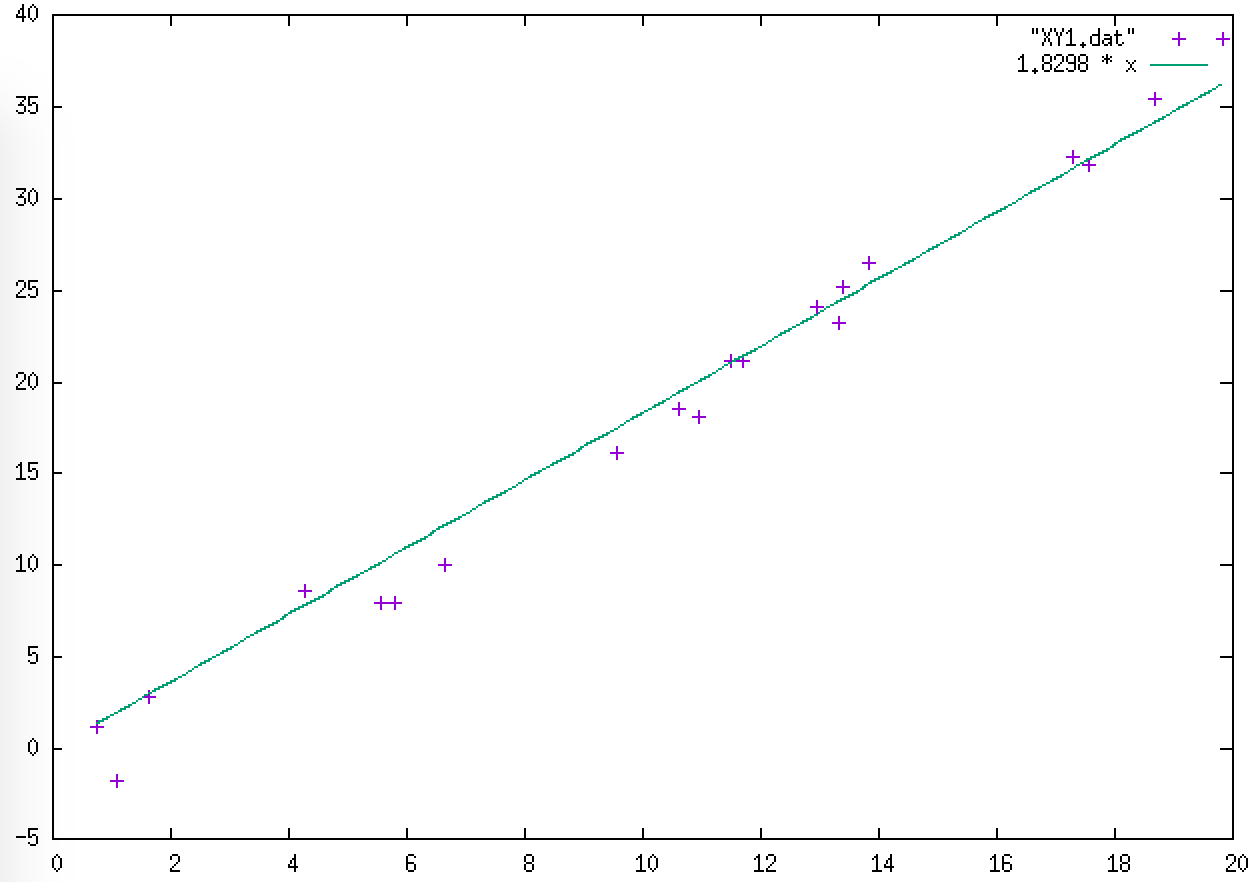
\includegraphics[width=0.6\linewidth]{plot/least_square/XY1.png}
		\end{figure}

		\item The example above is one-dimensional and trivial. A non-trivial multi-dimensional data set can be found in \ttt{X2.txt} and \ttt{Y2.txt}, where $\bm{x}^{(i)} \in \mathbb{R}^{5}$ and $\bm{y}^{(i)} \in \mathbb{R}^3$ and there are $20$ of them. If you do the math correctly, the least square loss as defined in eqn (\ref{eq:lsloss}) should be $3.431402129330746$.
	\end{enumerate}

\end{document}
